
%%%%%%%%%%%%%%%%%%%%%%% file template.tex %%%%%%%%%%%%%%%%%%%%%%%%%
%
% This is a general template file for the LaTeX package SVJour3
% for Springer journals.          Springer Heidelberg 2010/09/16
%
% Copy it to a new file with a new name and use it as the basis
% for your article. Delete % signs as needed.
%
% This template includes a few options for different layouts and
% content for various journals. Please consult a previous issue of
% your journal as needed.
%
%%%%%%%%%%%%%%%%%%%%%%%%%%%%%%%%%%%%%%%%%%%%%%%%%%%%%%%%%%%%%%%%%%%
%
\RequirePackage{fix-cm}
%
%\documentclass{svjour3}                     % onecolumn (standard format)
%\documentclass[smallcondensed]{svjour3}     % onecolumn (ditto)
%\documentclass[smallextended]{svjour3}       % onecolumn (second format)
\documentclass[twocolumn]{svjour3}          % twocolumn
%
\smartqed  % flush right qed marks, e.g. at end of proof

\usepackage{graphicx}
\usepackage{mdwlist}
\usepackage{nth}
\usepackage{todonotes}
\newcommand{\xap}{$X^2A_2'$ }
\newcommand{\bepa}{$B^2E'$ }
\newcommand{\bepb}{$B^2E'$ }

\newcommand{\superast}{\textsuperscript{$\ast$}}
\newcommand{\superdag}{\textsuperscript{$\dagger$}}

\graphicspath{{figs/}}

%\hyphenation{lib-Mesh Open-MP}

% In 2 column environments LaTeX often needs to be told to be less
% tolerant of overflow and more tolerant of overwide spacing
\sloppy

% please place your own definitions here and don't use \def but
% \newcommand{}{}
%
% Insert the name of "your journal" with
% \journalname{myjournal}
%
\begin{document}

\title{Experiences Porting Scientific Applications to the Intel “Knights
Landing” (KNL) Xeon Phi Platform} 
%\subtitle{Do you have a subtitle?\\ If so, write it here}

\titlerunning{Experiences Porting Scientific Applications to the Intel
“Knights Landing” (KNL) Xeon Phi Platform} 

% guys, please adjust order here any way you see fit....
\author{Nicholas~Malaya\superast \and D.~McDougall \and C~Michoski \and M~Lee}

\authorrunning{Nicholas~Malaya\superast \and D.~McDougall \and
C~Michoski \and M~Lee} % if too long for running head 

\institute{
              \superast{}Institute for Computational Engineering and Sciences
	      (ICES), 
	      The University of Texas at Austin \\
              \email{\{nick,damon,michoski,mk\}@ices.utexas.edu} \\
	      \\
%             \emph{Present address:} of F. Author  %  if needed
%           \and
           %K. Schulz \at
%	      \vspace*{5pt}
              \superdag{}Texas Advanced Computing Center and ICES \\
	      The University of Texas at Austin \\
              \email{karl@tacc.utexas.edu} ({\em corresponding author})   %  \\
}

%\date{Received: date / Accepted: date}
% The correct dates will be entered by the editor

\maketitle

\vspace*{-18pt}
\begin{abstract}

This paper presents experiences using Intel's KNL MIC platform on early-access
hardware for the upcoming Stampede 2 cluster launching in Summer 2017. We focus
on 1) porting of existing scientific software; 2) observing performance of this
software.  Additionally, we comment on both the ease of use of KNL and observed
performance of KNL as compared to previous generation ``Knights Ferry'' and
``Knights Corner'' Xeon Phi MICs~\cite{schulz2012early}.  Fortran, C, and C++
applications are chosen from a variety of scientific disciplines including
computational fluid dynamics, numerical linear algebra, uncertainty
quantification, finite element methods, and computational chemistry.
 
\keywords{co-processors \and heterogeneous computing \and scientific
  applications \and many integrated cores \and many-core architecture}

\end{abstract}

\section{Introduction}
\label{sec:intro}

Accelerators like current generation GPGPUs offer relatively high
floating-point throughput and memory bandwidth with a lower relative power
footprint than general-purpose compute platforms~\cite{gpu_hpc:2009}. However,
GPU-based acceleration commonly requires special programming constructs (e.g.
NVIDIA's CUDA language) for the accelerator to work.  Intel's Xeon Phi
many-core architectures offer a balance with a smaller core count than GPGPUs
but an x86 architecture and therefore don't need specialised programming
paradigms.  Existing MPI or OpenMP~\cite{openmp_standard} threaded Fortran, C,
or C++ codes can be compiled and run with relative ease.

The applications considered in this paper are taken from existing development
efforts within the PECOS Center at the University of Texas at Austin.  This
paper reports on two main areas: 1) the level of effort required in porting
software applications from a wide array of scientific disciplines written in
commonly used procedural languages; and 2) observed performance of these
applications.  The applications include Fortran, C, and C++ codes, and include
an example with no prior thread-based parallelism as well as codes with
existing OpenMP or MPI based threading from the following scientific
disciplines: 1) computational fluid dynamics; 2) uncertainty quantification;
3) computational chemsitry; and 4) finite element methods.

The remainder of the paper is organized as follows: \S\ref{sec:hardware}
describes the testing infrastructure, \S\ref{sec:cross_compile} describes cross
compiling experiences, \S\ref{sec:apps} presents results of the porting efforts
for each application considered, and \S\ref{sec:summary} summarizes the overall
experiences.

\section{Testing Infrastructure}
\label{sec:hardware}

The test hardware used for this exercise was the recent Stampede cluster
upgrade at the Texas Advanced Computing Center.  This upgrade cluster leaves
the original Stampede cluster hardware untouched and adds compute performance
capabilities with the newest iteration of Intel's MIC architecture codenamed
``Knights Landing''.

The ``Knights Landing'' Xeon Phi 7250 compute nodes in the Stampede Upgrade
cluster boast 68 cores, each with 4 hardware threads, are bootable and each run
a lightweight CentOS 7 Linux kernel.  They also have 16GB of high-bandwidth
Multi-Channel Dynamic Random Access Memory (MCDRAM) and 384GB of DDR4-2400.

The login node of the Stampede Upgrade (KNL) cluster is a 14 core (28 thread)
Haswell generation Intel Xeon E5-2695v3 processor with a clock speed of
2.30GHz.  This was used to cross-compile scientific applications for the KNL
compute nodes.  Applications were built with version 17.0.0 20160721 of Intel's
own C, C++, and Fortran compilers.

\section{Third Party Library Cross-Compiling}
\label{sec:cross_compile}

As with many scientific research groups, application development at the PECOS
center employs many open-source libraries.  Fortunately, TACC's module system
built on top of \texttt{lmod} provided many commonly used scientific packages
already compiled with the necessary instructions supported by KNL.  Moreover,
since the Stampede Upgrade cluster contains only bootable KNL nodes, the login
Haswell node is not needed for offloading computation.  We use it only for
compiling and building software.  Compilation is possible on KNL, but it is
much slower.

The following software pacakges were compiled for the KNL MIC architecture:
QUESO, ArcSyn3Sis, Poongback, C4, OCCA.

%Building these libraries for the host environment is a well supported, common
%task, but building them for MIC required cross-compilation.

% Building the libraries for MIC represents a new challenge as it necessitates
% cross-compilation techniques.  Fortunately, many of these libraries utilize the
% Autotools build system, which can support cross-compilation.  Native MIC builds
% were configured by specifying an existing non-native Linux host (e.g. {\em
% blackfin}) or by augmenting the autotools {\em config.sub} file with a new
% ``mic'' Linux target.  To build native libraries for MIC, the ``-mmic" flag was
% added to all relevant compiler flags.
%
% %For other packages, simply passing ``-mmic" to the compiler options was
% %sufficient to build a native MIC package.
%
% As an example, the following configure options were used to build a native MIC
% version of the FFTW 3.3 static library:
%
% \vspace*{-6pt}
% {\small
% \begin{verbatim}
% ./configure CC=icc CXX=icpc FC=ifort       \
%    CFLAGS="-mmic -O3" CXXFLAGS="-mmic -O3" \
%    FCFLAGS="-mmic -O3" --host=blackfin
% \end{verbatim}
% }
%
% These strategies successfully built native static libraries and executables for
% MIC. However, building shared libraries was more delicate and not always
% successful. For example, configuring Boost to build shared libraries caused the
% linker to crash.  Other shared libraries, such as GSL, built without incident.

\section{Applications and Scientific Kernels}
\label{sec:apps}

The subsections which follow highlight two things: 1) the level of effort
required in porting software applications from a wide array of scientific
disciplines written in commonly used procedural languages; and 2) observed
performance of these applications.  Applications are drawn from four distinct
scientific disciplines.

\paragraph{Poongback}  Poongback is a Fortran application targeted towards
solving the incompressible Navier-Stokes equations in a periodic wall-bounded
channel.

\paragraph{C4}  C4 is a collection of Fortran applications that leverages a
suite of algorithms for solving coupled-cluster problems in quantum chemistry.

\paragraph{QUESO}  QUESO is a C++ library for the Quantifying Uncertainty in
Estimation, Simulation, and Optimization.  It provides a suite of algorithms
for sampling unknown probability distributions and provides a parallel (MPI)
environment to allow the user to leverage this in large-scale engineering
applications.

\paragraph{ArcSyn3sis}  ArcSyn3sis is a C library that implements a
discontinuous Galerkin method that respects complex geometries.

We explore each of these applications in turn.

% DNS defined in the intro!
\subsection{Incompressible DNS FFT Kernel}
\label{sec:dns}

In many fluid dynamics applications, turbulence plays a
dominant role. Unfortunately, turbulence is notoriously complex and
difficult to model.  One reliable
tool for analyzing turbulence is direct
numerical simulation (DNS)\cite{jimenez:2007}, where Navier--Stokes numerical solutions
are fully resolved
in both time and space. 
%%%Although DNS is too
%%%computationally expensive for engineering calculations, high quality
%%%DNS is an excellent tool for investigation of turbulent flow physics.  

% However, the extremely high resolution requirements of DNS
% require excellent system performance. 
% Communication costs arise from large volume of data all-to-all exchanges
% between nodes needed to perform transposes. Direct matrix solves for the
% wall-normal component of velocity rely on processor clockspeeds. Due to
% the large problem sizes, the code is also memory intensive, and depends
% on memory bandwidth and cache size available; finally, writing large
% amounts of data for postprocessing makes I/O performance critical.

%The simulation code seeks the solution of the
%time-dependent three-dimensional incompressible Navier--Stokes
%equations. Periodic boundary conditions are imposed in the streamwise
%and span-wise direction, while in the wall normal direction, no slip
%conditions are imposed at the walls. A partially implicit third order
%Runge-Kutta/Crank--Nicholson scheme is used for time discretization. 
%In

In the DNS application used
by PECOS to simulate channel flow, a Fourier spectral
representation is used in the streamwise and spanwise directions,
while a high order compact finite difference is used in the
wall-normal direction\cite{KMM:87,Lele:92}.
%%%% picture of channel
%%%\begin{figure}[h]
%%%\begin{center}
%%% \includegraphics[height=.39\linewidth]{geometry}
%%% \caption{The Channel Geometry.}
%%%\end{center}
%%%\end{figure}
The Fourier method allows a natural decoupling between different modes
in transformed space such that multiple tasks can operate on their own data
independently. Our method uses a 2D decomposition which divides an $N_x
\times N_y \times N_z$ domain into M pencils. Fourier transforms in 3D
are performed one direction at a time, and transposes 
re-partition the domain into pencils aligned in appropriate
directions,
as depicted in Figure~\ref{fig:pencil2}. This
paper focuses on single-node performance.  Thus,
for the kernel discussed below, the final pencil depicted (x,z,y) is
the portion of the domain considered for FFT analysis on MIC.

% picture of pencils
\begin{figure}[htb]
 \begin{center}
  \includegraphics[width=0.35\textwidth]{PencilTransposeSchematic}
  \caption{The two dimensional data decomposition. The localized FFT
    on the pencil shown on the far right is ported to the KNF MIC platform.}
    \label{fig:pencil2}
 \end{center}
\end{figure}

Algorithmically, the final inverse Fourier transform, physical space
calculations, and the first Fourier transform into wavespace are
performed completely on-node and do not require MPI subroutine calls. 
Previously the inverse Fourier transform, realspace calculations,
and forward transform were performed separately. This section of code
was re-factored to perform all three steps on each line of the pencil
individually. These changes improved cache coherency and optimized the
algorithm for multithreading, the performance and scaling of which is
the basis for this section. 

The resulting FFT kernel was run with a pencil size of $\{N_x,N_z, N_y\} =$ 
(8192,1280,1), with $N_x$ corresponding to the direction being
Fourier transformed. This was iterated over six pencils to emulate
the real DNS code, which requires operating on three velocity components
($u$,$v$,$w$) as well as the non-linear terms ($uu$,$uv$,$ww$) required
to resolve the velocity at the subsequent timestep. The size of the
pencil was chosen to correspond to a realistic pencil size for a a
single compute node during a large scale DNS simulation, where the
global mesh size would be (8192,12288,1024). 

The kernel application code is written entirely in Fortran-90, and
uses OpenMP for multithreading to perform multiple 2D
FFTs simultaneously.
%and requires a series of
%two-dimensional FFTs to complete the analysis.  

We compare results from FFTW 3.3 to the FFTW interface in MKL.  Runs
were made at various thread counts on both the host Westmere and KNF
MIC platforms and the results were verified analytically. Timings were
averaged over two successive runs, and results comparing FFTW to MKL
performance are shown in
Figure~\ref{fig:mkl-vs-fftw}. Figure~\ref{fig:mkl-vs-fftw}(a) compares
the speedup factor obtained using MKL on Westmere with observed
performance increases ranging from $\sim$20-40\%.
Figure~\ref{fig:mkl-vs-fftw}(b) shows results on MIC, where the
performance increases with MKL are more dramatic, suggesting that the
FFT implementation within MKL enables more vectorization than the FFTW
counterpart. This performance difference also impacts scalability on
MIC, as shown in Figure~\ref{fig:dns_scaling}.  In this case, the
speedup factor is based on a baseline case with four threads.  The MKL
implementation scales much better than the FFTW version. With 120
threads, an overall scaling efficiency of 72\% was achieved using MKL,
whereas only 35\% was achieved with FFTW.

% completed on both the
%FFTW for Fourier transforms. The code is
%essentially a series of DO loops that iterate over the z and y
%directions. 

To quantify the impact of various runtime affinity settings available
on MIC, Figure~\ref{fig:dns_affinity} presents the real-to-complex
(Fourier transform into frequency space) performance gains for several
thread affinity options: scatter, compact or
explicit. Results in Figure~\ref{fig:dns_affinity} are
all compared against the default case: no KMP\_AFFINITY setting.
For both MKL and FFTW
linkage, the {\em scatter} setting provided the best overall
performance across a wide thread-count range.  Note that this
setting was seen to have a significant impact on observed runtimes.

%% From the provided Intel
%% documentation:
%% \begin{itemize}

%%  \item \textbf{Scatter}: ``Specifying scatter distributes the threads as
%%        evenly as possible across the entire system. scatter is the
%%        opposite of compact; so the leaves of the node are most
%%        significant when sorting through the machine topology map.'' 

%%  \item \textbf{Compact}: ``Specifying compact assigns the OpenMP thread
%%        $\langle n \rangle + 1$ to a free thread context as close as
%%        possible to the thread context where the $\langle n \rangle$
%%        OpenMP thread was placed.''

%%  \item \textbf{Explicit}:``Specifying explicit assigns OpenMP threads to
%%        a list of OS proc IDs that have been explicitly specified by
%%        using the proclist$=$ modifier, which is required for this affinity
%%        type. ''
%% \end{itemize}



% need to add discussion of affinity results here
% http://software.intel.com/sites/products/documentation/studio/composer/en-us/2011/compiler_c/optaps/common/optaps_openmp_thread_affinity.htm#Explicitly_Specifying_OS_Proc_IDS__GOMP_CPU_AFFINITY 

\begin{figure}[htp]
\begin{center}
\includegraphics[width=0.95\linewidth]{dns_westmere_fftw_vs_mkl.pdf}
(a)
\includegraphics[width=0.95\linewidth]{dns_mic_fftw_vs_mkl.pdf} 
(b)
\end{center}
\vspace*{-.5cm}
\caption{Relative comparison between threaded FFT kernel
  used in DNS applications on (a) dual-socket Westmere server and (b)
  KNF MIC co-processor.}
\label{fig:mkl-vs-fftw}
\end{figure}

\begin{figure}[h]
\begin{center}
\includegraphics[width=0.9\linewidth]{dns-fftw-scaling.pdf}
\end{center}
\vspace*{-.5cm}
\caption{Scaling of DNS FFT kernel on KNF MIC accelerator ({KMP\_AFFINITY=scatter}).}
\label{fig:dns_scaling}
\end{figure}

\begin{figure}[htp]
\begin{center}
\includegraphics[width=1.0\linewidth]{dns_affinity_mkl.pdf}
(a)
\includegraphics[width=1.0\linewidth]{dns_affinity_fftw3.pdf}
(b)
\end{center}
\vspace*{-.5cm}
\caption{Influence of runtime affinity setting on MIC.
  Relative performance change is based
  on comparison to runs with no affinity setting provided. A
  positive performance change indicates faster runtimes.  Results are
  presented for FFTs performed with the (a) MKL and (b) FFTW3
  libraries.}
\label{fig:dns_affinity}
\end{figure}




%

%\begin{figure}[htp]
%\begin{center}
%\includegraphics[width=1.0\linewidth]{dns_full_kernel.pdf}
%\end{center}
%\vspace*{-.5cm}
%\caption{Scaling of the Complex-to-Real FFT, Nonlinear computations and
% Complex-to-Real FFT DNS kernel on KNF MIC accelerator.}
%\label{fig:dns_scaling}
%\end{figure}
%

% DNS defined in the intro!
\subsection{Incompressible DNS Application}
\label{sec:dns_full}

In many fluid dynamics applications, turbulence plays a
dominant role. Unfortunately, turbulence is 
notoriously complex and difficult to model. Even though the governing equation, Navier-Stokes equation, for the turbulent flow is well-defined, the understanding of turbulent flow is still a challenging problem. One of the reason why it is difficult to study is that the length and time-scale of turbulent flow becomes smaller as Reynolds number $Re$ increases. ($Re$ the ratio of inertia force to viscous force of flow.) In Direct numerical simulation (DNS) one allocates grids as many as necessary, and the necessary grids size increases as $Re$ increases. As far as we know the largest wall-bounded DNS is performed by (Lee \& Moser 2015, JFM) and 240 billions degree of freedom has been used for the flow between parallel planes at $Re = 250000$. However, higher $Re$ simulation with larger problem size is required to answer many unsolved problems in fluid dynamics. Hence, it is natural to prepare the simulation code for next generation computers.

Poongback, the DNS code for incompressible channel flow, has already shown excellent performance and has been already used in several researchers. Especially, it has been used for the simulation by (Lee \& Moser 2015, JFM) and generating the data for virtual flow laboratory in Johns Hopkins Turbulence Data Base (Cite here). The spectral-Galerkin method and B-spline collocation method are used in PoongBack. There are four main parts in Poongback, data transpose with 2D decomposition, multiple 1D FFTs, solving linear equations with real matrix and complex vectors and I/O in HDF5 format. For I/O, we uses customized I/O library, ESIO, but we have not tested its performance for this work. The data transpose 2D decomposition and multiple 1D FFTs are done by FFTW3.3 library. Note that FFTW3.3 (and above) library support the use of MPI but it is implemented for 1D data decomposition. To overcom this issue, we created two MPI-subcommunicators, and called FFTW for data transpose and FFTs seperately. Also, we have implemented customized banded-matrix solver to linear equations. See (Lee, Malaya, Moser 2013, SC) for more detail about PoongBack.

\begin{figure}[htb]
 \begin{center}
   \includegraphics[width=0.45\textwidth]{DNS_FFT_WAVE}
   \caption{Strong scaling result of 1D FFTs and Solving N-S equations in wavespeace for single timestep.}
   \label{fig:DNS_strong_scale_fft_wave}
 \end{center}
\end{figure}

For this study the grid size is used $1024\times128\times512$ and the grid size is comparable for $Re_\tau = 180$ simulation by (cite here). Throughout the every benchmark cases, the MCDRAM is used as a cache memory between processors and DRAM. Figure~\ref{fig:DNS_strong_scale_fft_wave} shows the strong scaling performance of 1D FFTs (real-to-complex, complex-to-real and complex-to-complex) and floating point operations with complex numbers including linear equation solvers. The linear equation, $A\mathbf{x} = \mathbf{b}$, is solved to compute B-spline coefficients. $A$ is a diagonal dominant banded matrix with additional non-zero elements in several top and bottom rows. $\mathbf{x}$ and $\mathbf{b}$ is complex vectors. As shown in the Figure~\ref{fig:DNS_strong_scale_fft_wave}, FFTs and floating point operations shows good scalability in both OpenMP only and MPI only cases with upto 64 processors. Using MPI only shows slightly better performance but the difference is negligible. After the hyperthread\todo{it this right term?} is used performance with FFTs are decreased because FFTs are bounded by the memory access not by floating point operations. On the otherhands, the kernel with linear equation shows slight performance increases even with the hyperthreads. Interestingly, using MPI shows better performance than OpenMP. This maybe due to the difference of memory access pattern between two parallelism. \todo{Chris, is this make sense?}.


\begin{figure}[htb]
 \begin{center}
   \includegraphics[width=0.45\textwidth]{DNS_Transpose}
   \caption{Strong scaling result of data reorder and MPI communication; OpenMP is not used.}
   \label{fig:DNS_strong_scale_transpose}
 \end{center}
\end{figure}

\begin{figure}[htb]
 \begin{center}
   \includegraphics[width=0.45\textwidth]{DNS_Parallelism}
   \caption{Comparison of MPI$\times$OpenMP configuration}
   \label{fig:DNS_MPI_OpenMP}
 \end{center}
\end{figure}

\begin{figure}[htb]
 \begin{center}
   \includegraphics[width=0.45\textwidth]{DNS_full_timestep}
   \caption{Strong scaling result of total elapsed time for single timestep; (MPI tasks $\times$ OpenMP threads) is hybrid configuratation which showed  the best performance.}
   \label{fig:DNS_strong_scale_total_elapsed_time}
 \end{center}
\end{figure}





\todo{if we merge this with the previous section, we can have an intro
to dns and then talk about each in detail}


% DNS defined in the intro!
\subsection{Cholesky Factorization}
\label{sec:chol}


Decomposition of PD matrix into the product of a lower triangular matrix
and its conjugate transpose.

%
% NM --- feel free to disregard anything I recommend here
%

\missingfigure{Strong scaling on single MIC (e.g. problem size constant
and increasing number of threads)}
% DNS defined in the intro!
\subsection{Blended Isogeometric Discontinuous Galerkin (BIDG) Method}
\label{sec:isogeometric}

For the scaling study the blended isogeometric discontinuous Galerkin (BIDG) code, ArcSyn3sis was used.  The BIDG algorithm was developed in \cite{Michoski2016658}. to exploit and seamlessly merge key capabilities offered by both isogeometric analysis and discontinuous Galerkin methods. This method is an inherently high-order method that is amenable to $hp$-adaptive schemes, and shows requisite super-exponential convergence behaviors.

In traditional isogeometric analysis tight coupling between computer aided design (CAD) mesh automation tools for complex geometric domains, such as jet engines and tokamak fusion reactors, has been developed for triangles in two dimensions  \cite{Engvall2016378}, and semi-arbitrary elements in three dimensions \cite{EngvallPress}.  This allows for meshes that exactly preserve the underlying geometry of real-world mesh designs, including arbitrarily smooth and discontinuous features.  In many application, geometric sensitivities are known to dominate errors, and as such having high-order accurate solutions on geometrically consistent meshes is essential.


\begin{figure}[h]
\begin{center}
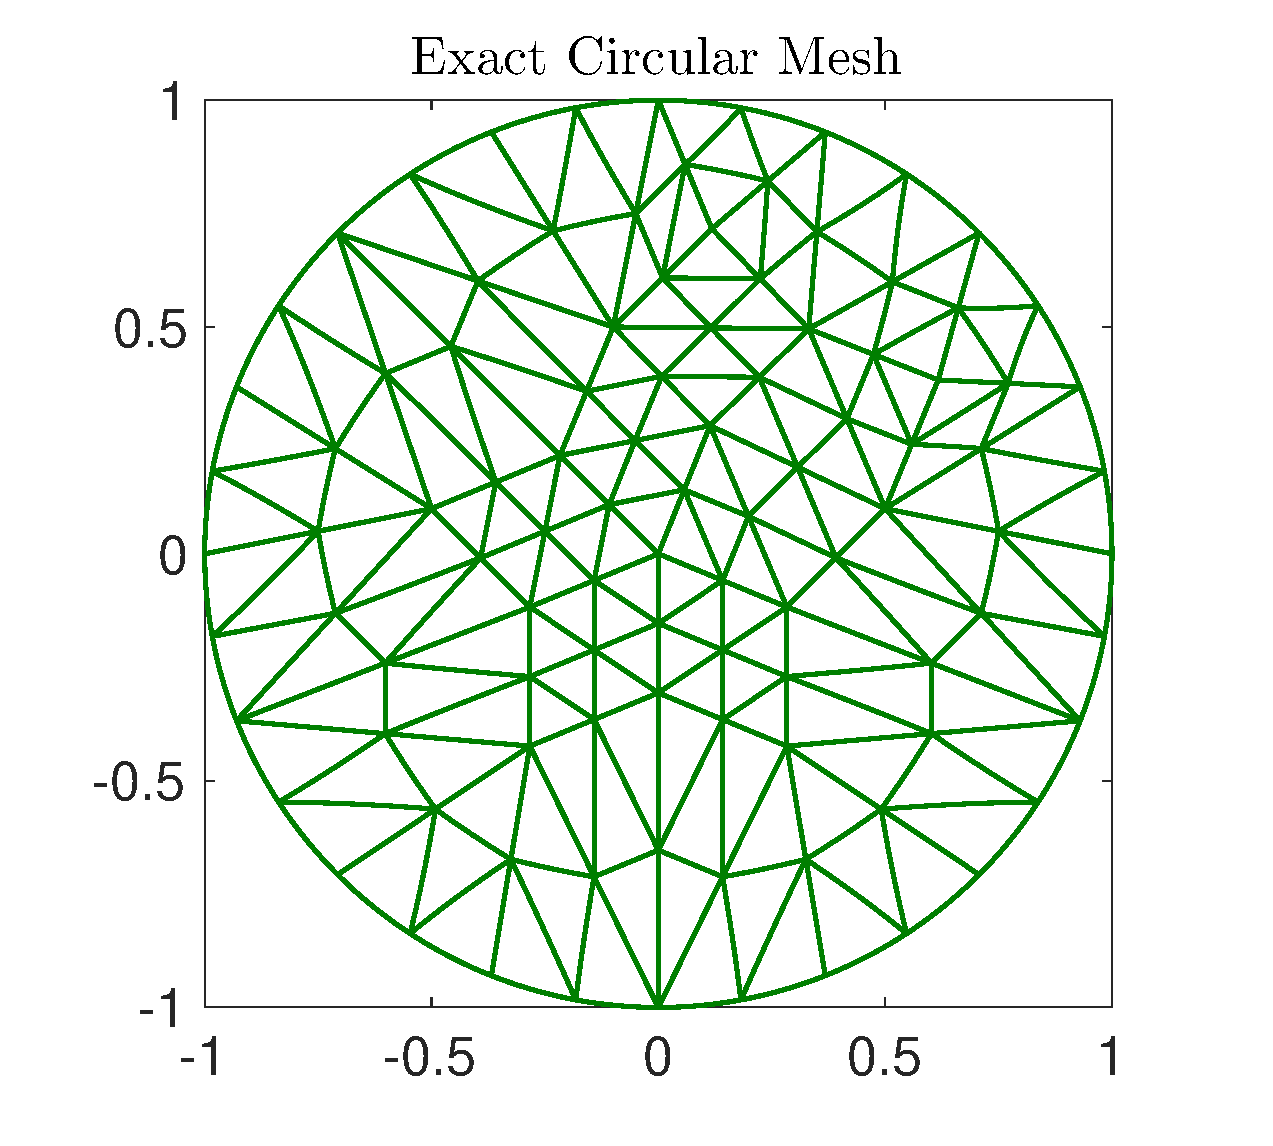
\includegraphics[width=0.8\linewidth]{./bidg_data/168_circ}
\end{center}
\vspace*{-.5cm}
\caption{Exact b\'{e}zier circular mesh used in the scaling study.}
\label{fig:dns_scaling}
\end{figure}


The discontinuous Galerkin method, on the other hand, excels in aspects of its computational efficiency in the context of modern architectures, particular in convection-dominated flows that allow for localization of finite element stencils in such a way that dynamic problems lead to block diagonal matrix systems.  The locality of the memory footprint in these application models leads to the ability to compute at high local order at unusally high arithmetic intensity \cite{Klöckner2009786}.

The BIDG method merges these two methods seamlessly by utilizing a peicewise rational isogeometric basis for the geometry, and a peicewise discontinuous polynomial representation for the model, while providing an exact (and properly conditioned) geometric transformation between the two spaces  \cite{Michoski2016658}.

For our scaling test here we solve the first-order acoustic wave equation: \begin{equation} \label{awe} \frac{\partial p}{\partial t} + \nabla\cdot \boldsymbol{u} = 0, \quad  \frac{\partial\boldsymbol{u}}{\partial t} + \nabla p = 0, \end{equation} where $\boldsymbol{u}=(u_x,u_y)$ is the velocity, and $p$ the pressure.

Broadly such a system is discretized by solving the semidiscrete block diagonal system \[ \left( v, \frac{ \partial A}{\partial t} \right)_{\Omega_{i}}= V_{\Omega_{i}}+S_{\partial\Omega_{i}} \] for $A = (p,\boldsymbol{u})$, $V_{\Omega_{i}}$ a volume kernel that has only elementwise dependencies, and $S_{\partial\Omega_{i}}$ a surface kernel that depends on interelement communication through classical upwinding \cite{Michoski2014898}.  


\begin{figure}[h]
\begin{center}
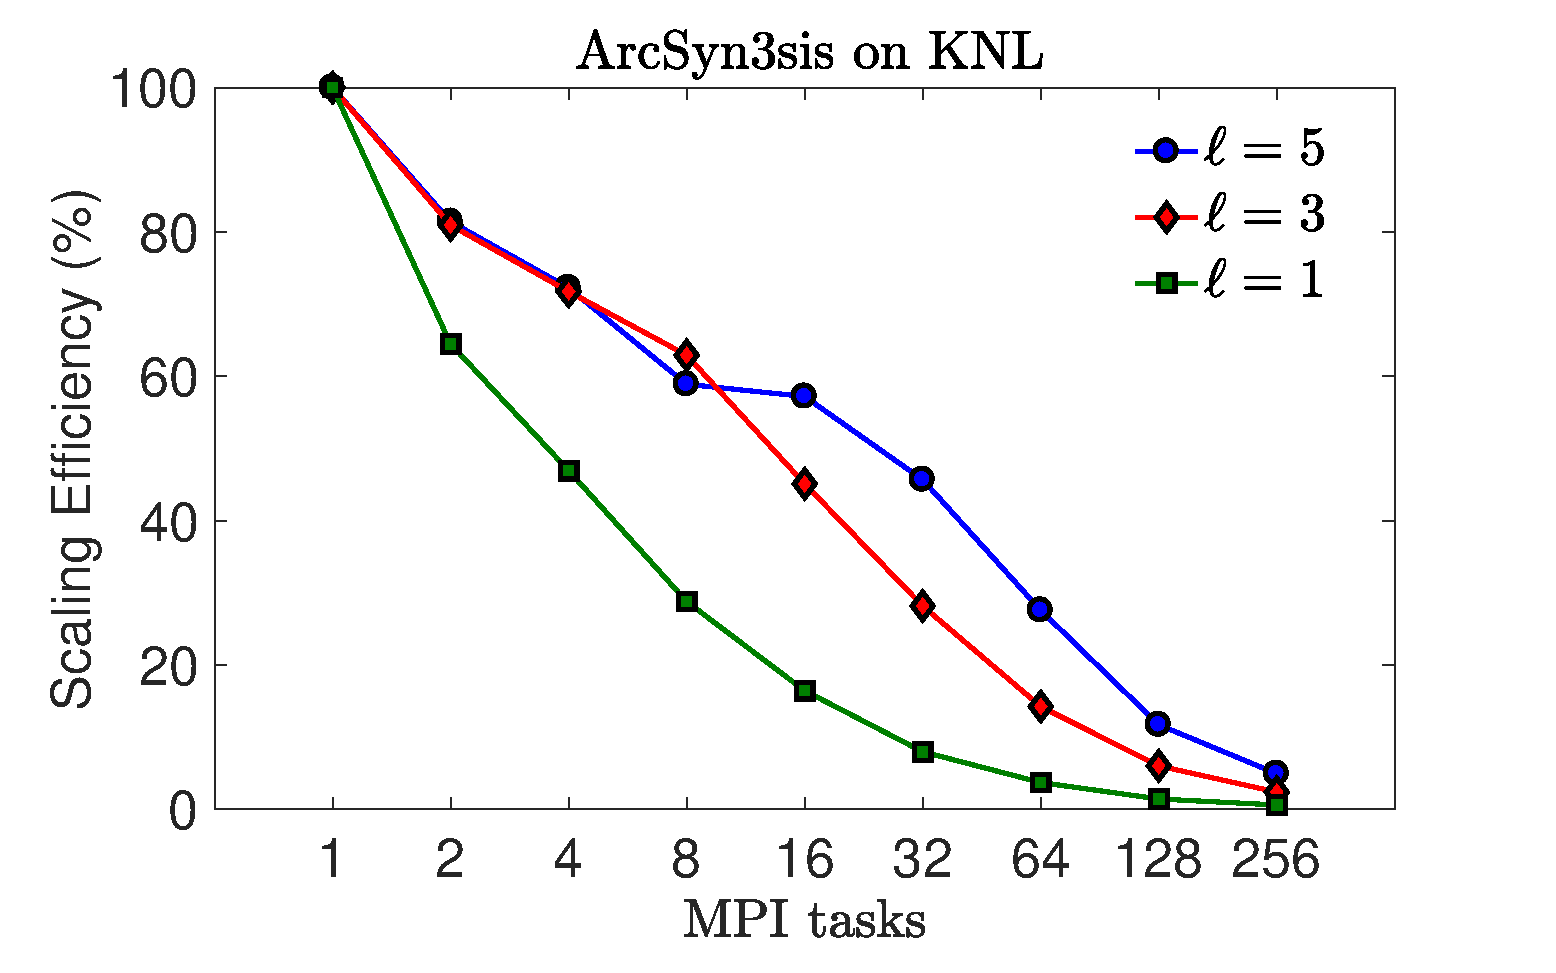
\includegraphics[width=0.95\linewidth]{./bidg_data/scaling_p}
\end{center}
\vspace*{-.5cm}
\caption{Strong scaling of the ArcSyn3sis BIDG kernel on KNL nodes run on isogeometric 168 element mesh, and shown at different element order $\ell$.}
\label{fig:bidg_scaling}
\end{figure}


The implementartion on isogeometric meshes utilizes the Open Concurrent Compute Abstraction (OCCA) library \cite{MedinaPress}.  The library uses an offload model for abstracting back-ends and kernel libraries from OpenMP, OpenCL, and CUDA using a macros C-based approach.  The OCCA kernel implements macro-based just-in-time code generation so that the platform target can be identified at runtime.  Threaded barriers are also set in the application kernel to allow for thread-based granularity, giving more flexibility in the optimization procedure.  The implementation of the ArcSyn3sis kernel allows for aliasing of in the flattened arrays, such that the data structures can be called more intuitively (e.g. a 4-tensor can be called as a four array, instead of indexed as a flattened continguous one array).  The volume kernel can be written in three nested loops, and outer loop over elements, and two inner loops over the degrees of freedom of the DG basis.  The surface kernel similarly loops over elements, but then due to an added interpolation step coming form the isogeometric transformation, extends one of these nested loops over the quadrature degrees of freedom for curved edges instead.

The results of the basic scaling study are shown in Fig.~\ref{fig:bidg_scaling}.  These priliminary results seem to indicate improved scaling as function of polynomial order, which is consistent with the theoretic algorithmic intensity of DG algorithms.  However, this is clearly not enough evidence to be certain that such scaling is being observed.  In particular, on this mesh we see an efficiency saturation above $\ell>5$.  Moreover, since the mesh itself has only 168 elements, the number of threads eventually exceeds the number of elements, making for some intriguing questions regarding the observ3ed behavior.  In order to fully understand this behavior, a more thorough study will be required,  including a streams benchmark \cite{McCalpin1995} and roofline performance test \cite{Williams:2009:RIV:1498765.1498785}.


%
% NM --- feel free to disregard anything I recommend here
%
 %yar\todo{Discuss, broadly, what class of problems this resides in and why humanity works on it}

%% yar2\todo{some basic intro to the linear algebra you are doing}

%% yar3\todo{any nuances of porting to MIC?}

%% yar4\todo{discussion of scalability observed}

%% \missingfigure{Strong scaling of the GPs on a single MIC (e.g. problem size constant
%% and increasing number of threads)}

%Finally, some discussion is needed: is DG ameniable to MICs? Vs typical CPUs? I
%naively guess so, since you can essentially vectorize several of the
%activities.


\section{Summary}
\label{sec:summary}

%
% achtung! old writing here
%
Overall, porting a number of different scientific applications and
kernels to the KNL architecture was 
%\todo{update this too!}
straightforward. Successfully ported applications (written in either
Fortran or C++) include serial codes as well as codes with existing
OpenMP based threading. Even native compilation of 3rd-party
libraries was reasonably straightforward, with only a few
configuration options left unsupported and dynamic library builds not
successful across all of the libraries considered.
%uniformly supported.

Performance results vary more widely.
We have demonstrated good strong scaling to large thread counts for some of our computational
kernels, but others only effectively used a fraction of the MIC's
potential capability.  However, runtime performance seldom degraded
for large thread counts on all workloads, and simple changes to
thread algorithms or affinity settings often delivered further
improvements.  Different workloads require different settings in order
to achieve peak performance. Finally, vectorization is critical to
fully exploit the MIC architecture. 


\begin{acknowledgements}
The Author's acknowledge the Texas Advanced Computing Center (TACC) at The
University of Texas at Austin for providing HPC resources that have
contributed to the research results reported within this paper.
\end{acknowledgements}

%\newpage
% BibTeX users please use one of
\bibliographystyle{spmpsci}      % mathematics and physical sciences
\bibliography{paper}   % name your BibTeX data base

\end{document}
% end of file template.tex

